\documentclass{article}

\usepackage{packages}
\usepackage{environments}
\usepackage{commands}

\begin{document}

\title{Typing Analysis}
\author{Dima Trushin}
\date{}
	
\maketitle
\tableofcontents

\section{General information}

The application uses Qt environment as an ecosystem. It does not use RTTI but uses exceptions. All components of the program must be inside NSApplication namespace. Nested namespaces should be placed in a subfolder of the project.

\subsection{Addressable objects}

I use term addressable object. It means an object that can be referenced by other objects. There are several types of addressable objects:
\begin{enumerate}
\item QObject
\item CApplicationImpl
\item Observer/Observable (TO DO)
\end{enumerate}
Addressable objects must be created on heap via \verb"std::make_unique" or similar mechanism. An exception to this rule: you may create an addressable object inside another addressable object.

\subsection{Exceptions}

The strategy is to catch exception, show a message, and die. Since Qt environment is not totally exception safe, it is not allowed to throw exceptions in an event loop. If a QObject requires to throw an exception and terminate the program it catches the exception by itself and then sends a signal to CQtLoopException object. CQtLoopException shows a message and stops the event loop. CQtLoopException is a singleton, it uses CAnyGlobalAccess template (see~\ref{section::Singleton}).

\section{Application Structure}

\subsection{Overview}

CApplication object initialize all required resources for the application including the ones to interact with Qt ecosystem. It may throw an exception while constructing. In order to minimize stack usage CApplication contains \verb"std::unique_ptr" to CApplicationImpl (it is addressable object). CApplicationImpl consists of four parts:
\begin{enumerate}
\item \textbf{CApplicationGlobals}. Its purpose is to initialize global resources, e.g., timers, loggers, thread pools, etc. Application initializes all global resources (basically singletons) at the start. This allows not to wast time on the first call. Also, it is inconvenient to initialize timers via the first call.
\item \textbf{CApplicationKernel}. Its purpose is to initialize the kernel of the application. The kernel does not depend on the GUI and uses MVC via observer pattern to interact with GUI.
\item \textbf{CApplicationGUI}. Its purpose is to provide View wrappers over Qt resources compatible with MVC pattern.
\item \textbf{CApplicationImpl}. Its purpose is to connect the kernel and the GUI via MVC.
\end{enumerate}
The order of construction is ensured by the inheritance mechanism.
\begin{center}
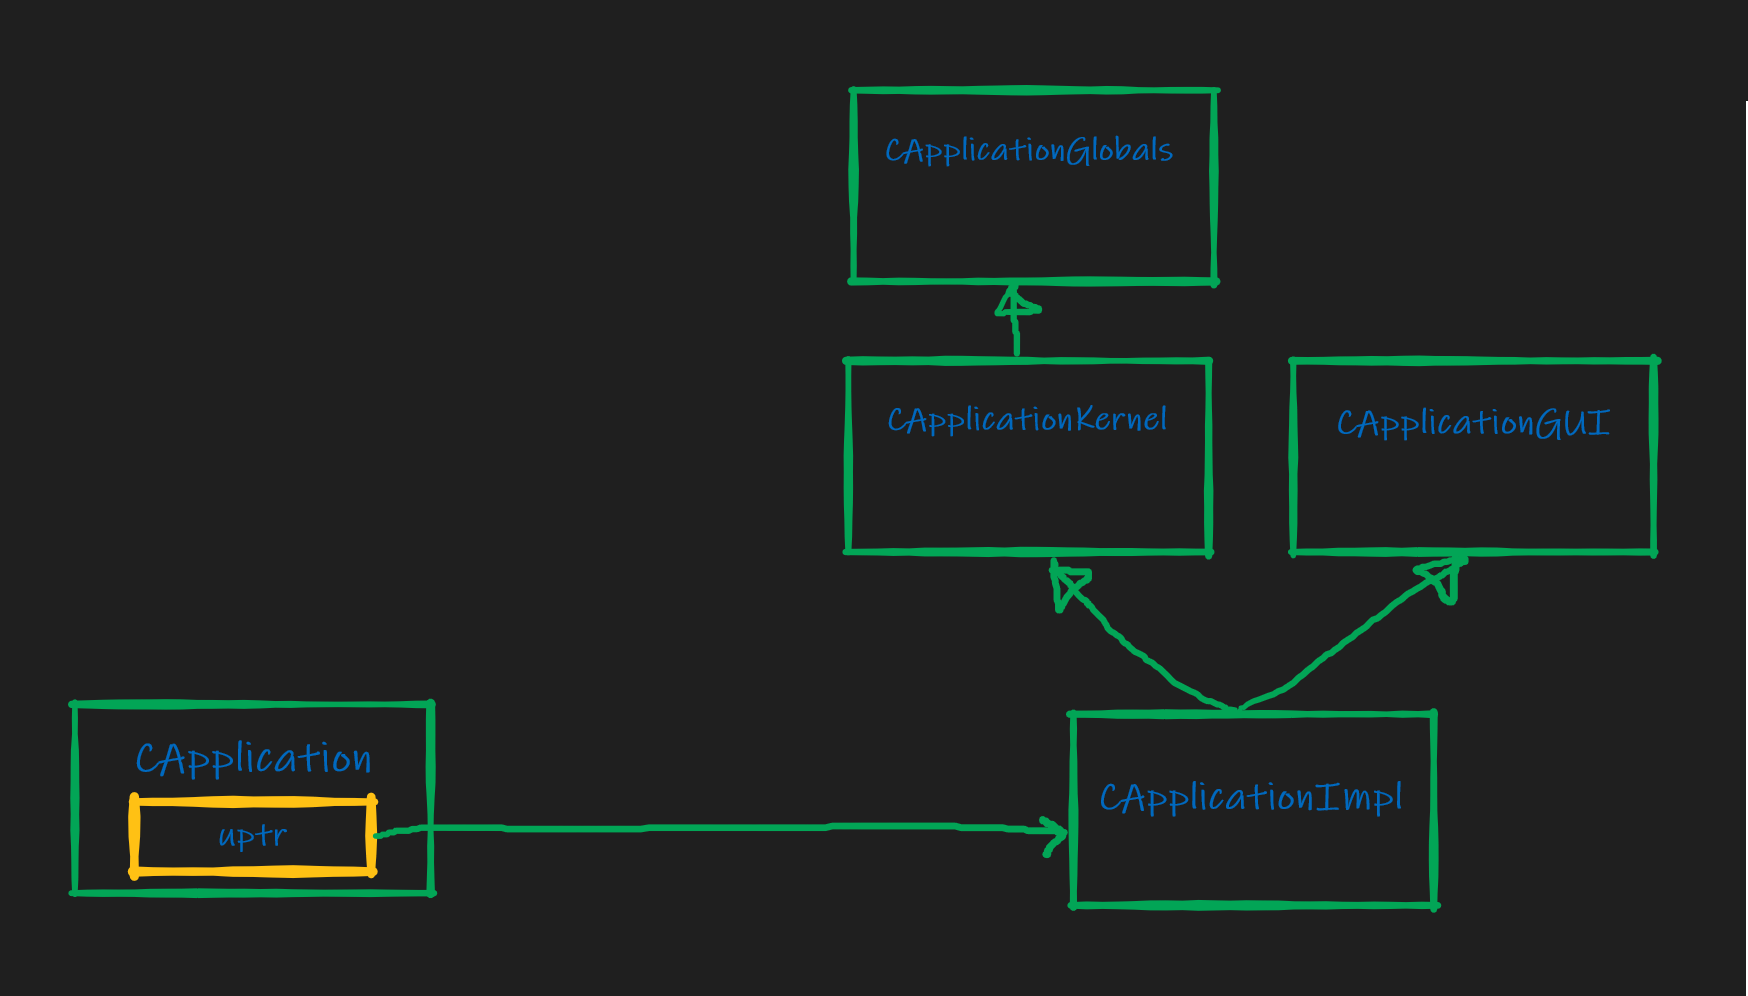
\includegraphics[scale = 0.3]{Figures/CApplicationStructure.png}
\end{center}

\subsection{Keyboard}

Each key on a keyboard has its position identifier \verb"CKeyPosition" and a key identifier \verb"CKeyId". CKeyPosition points out a physical location on a keyboard (e.g. a row and a column where the key is located). CKeyId identify the key depending on the keyboard layout (qwerty, Dvorak, etc.) CKeyPosition is an enum with following identifiers (xkb identifiers):
\begin{center}
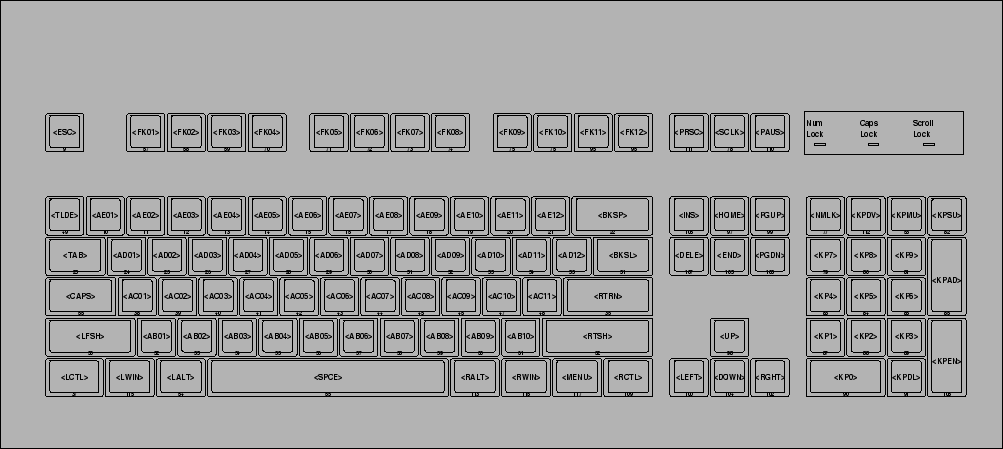
\includegraphics[scale = 0.5]{Figures/KeyPosition.png}

The picture is taken from \href{https://www.charvolant.org/doug/xkb/html/node5.html}{here}
\end{center}
It should be noted that the numeric values of the identifiers are slightly different from the one in xkb.

\subsection{Keyboard Interception}

The application must intercept keyboard events system-wide even if application is on the background. Qt ecosystem does not allow doing this. Hence, we need to implement our own mechanism. System wide interception usually means raw keyboard data is being intercepted. Hence, we need to implement translation of the key events to generated text. The main problem here is dead keys and ligatures. Current implementation supports dead keys but not ligatures (but the design allows to extend implementation to ligatures). Since system-wide interception must be done on the level of current OS, we implement these mechanism separately for each supported OS. Currently list of the supported OS
\begin{enumerate}
\item Windows 8 or higher.
\item Linux with X11 (there is a working prototype, not implemented yet, need to specify all the details).
\item macOS 10.14 (Mojave) or higher (there is a working prototype, not implemented yet, need to specify all the details).
\end{enumerate}

\paragraph{Current design}

\verb"CKeyboardHandler" serves as an object receiving all key events in a system independent form. This is a singleton described in section~\ref{section::KeyboardHandler}.

Let us consider the following figure:
\begin{center}
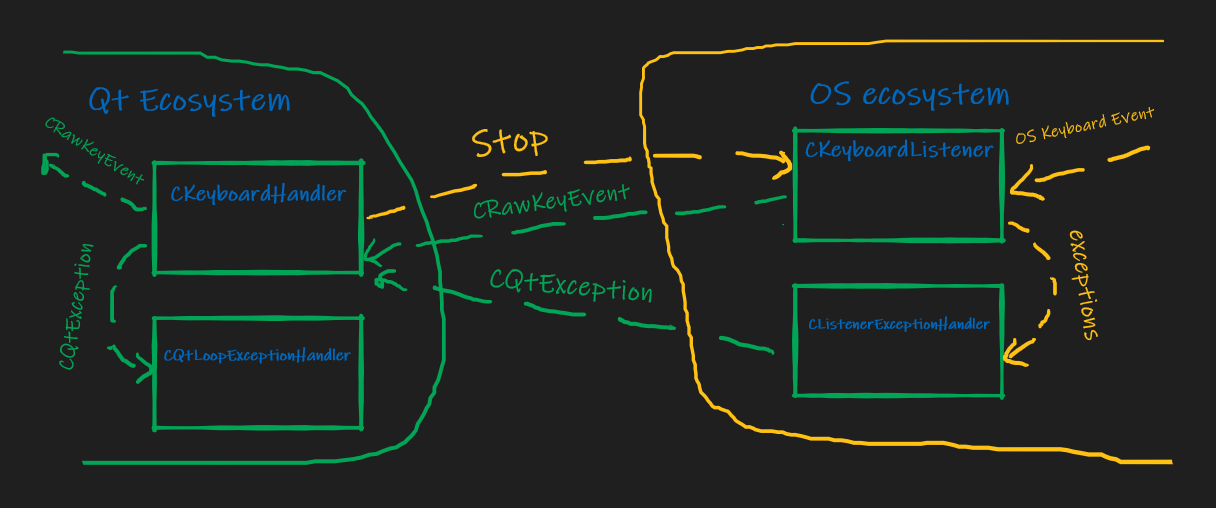
\includegraphics[scale = 0.5]{Figures/KeyboardInterception.png}

Green arrows represent queued Qt signals and yellow arrows represent OS dependent signals.
\end{center}

\verb"CKeyboardHandler" acts on the main GUI thread. It lives in Qt ecosystem and spawns an additional thread while construction. This additional thread lives in the ecosystem of OS. The main object acting on the additional thread is \verb"CKeyboardListener". Its roles are:
\begin{enumerate}
\item Intercept key events system-wise
\item Extract all the information from OS key events and translate it to OS independent form.
\item Resend OS independent key events to \verb"CKeyboardHandler" via Qt event system.
\item It receives only one message from \verb"CKeyboardHandler" via OS ecosystem message system. This is a ``stop'' message. Receiving the message it stops the additional thread.
\end{enumerate}

The second object acting on the additional thread is \verb"CListenerExceptionHandler". Its roles are:
\begin{enumerate}
\item Extract exception information.
\item Resend special exception messages to \verb"CKeyboardHandler".
\end{enumerate}
If an exception happens the event loop on the additional thread stops. \verb"CKeyboardHandler" resend the message to \verb"CQtEventLoopExceptionHandler". The latter one shows the error message and terminates the program.

\subsection{System independent Key event}

The \verb"CKeyEvent" contains the following information (TO DO not implemented, subject to change):
\begin{enumerate}
\item Pressing time.
\item Releasing time.
\item \verb"CKeyPosition" is an identifier of the Key position on the keyboard (independent on the layout this is a physical instance of a key).
\item \verb"CKeyId" is an identifier of a Key depending on layout. It is based on Windows Virtual Key table.
\item Key label. This is a symbol giving a human readable name for a key. For example, a letter or a number written on a keyboard, or a special symbol for system keys like shifts, backspace, enter, etc.
\item Key Text. This is a sequence of symbols appearing after pressing this key. It can be $0$, $1$, or $2$ symbols. The exact rules are explained below.
\item Flags (subject to change). These flags are reserved and can be needed to pass some additional information.
\end{enumerate}

\verb"CKeyboardHandler" receives the following structures from \verb"CKeyboardListener":
\begin{enumerate}
\item \verb"CKeyPressing".
\item \verb"CKeyReleasing".
\end{enumerate}

The structure \verb"CKeyPressing" contains the following fields:
\begin{enumerate}
\item \verb"CTime" The pressing time of the key.
\item \verb"CKeyPosition" The OS independent position of the key.
\item \verb"CKeyID" The OS independent ID of the key.
\item \verb"QChar" The key label. This symbol is shown on the keyboard.
\item \verb"QString" The text generated by the key.
\end{enumerate}

The structure \verb"CKeyReleasing" contains the following fields:
\begin{enumerate}
\item \verb"CTime" The releasing time of the key.
\item \verb"CKeyPosition" The OS independent position of the key.
\item \verb"CKeyID" The OS independent ID of the key. (subject to change, probably need to exclude this)
\end{enumerate}

When we need to pair the pressing and releasing events into one key, we identify the key by its position. It should be noted that the ID of the key can change. For example, if we press a number on the numpad (keep pressing), then press NumLock, and only then release the numpad number key, the numpad key will have different IDs while pressing and releasing. This happens because NumLock changes the mapping for physical keys to the corresponding IDs.

\subsection{Key mapping}

This section is mostly influenced by a \href{http://archives.miloush.net/michkap/archive/2006/03/23/558658.html}{series} of blogs by Michael S. Kaplan. His posts explain all subtleties of the keyboard handling on Windows. However, the principals he explains are applicable to any keyboard handling on any OS.

We separate keys to the following  categories:
\begin{enumerate}
\item Producing symbols keys (not necessarily printable symbols).
\item Shifters. These are: Shift (left, right), Ctrl (left, right), Alt (left, right), Capslock.
\item Ignorable. All other keys.
\end{enumerate}
The key Capslock has a toggled state. Also NumLock and ScrollLock have toggled state but we ignore them.

The symbol appearing on the screen depends on the sequence of keys pressed and not just one key. There are several reasons for that: dead keys or chained dead keys. I am currently focused on the dead key handling but keep in mind chained dead keys and other possible features for the future implementation. In order to handle a key pressing we need to know:
\begin{enumerate}
\item Key.
\item Shifters.
\item Layout.
\end{enumerate}

These triples may be classified as follows:
\begin{enumerate}
\item Undefined. This combinations do not produce any symbols and are ignored by symbol producing system.
\item Control. This combinations do not produce any symbols and are ignored by symbol producing system. However, this combinations may copy and past some text. We cannot handle these events and just ignore them. They are usually combinations of Ctrl or Ctrl+Shift with some other keys.

\item Printable Key. This keys usually produce a single symbol. There are cases when they produce a ligature, that is, a sequence of two UTF-16 characters combined into one symbol on print (ligatures currently are not supported but the support is possible).
\item Printable Dead Key. This are special keys. They do not produce symbol on its own but can be combined with other keys if compatible. A symbol producing system has a special buffer to store a previous dead key. This dead key is flushed from the buffer if the symbol producing system accepts one of the next keys. Theoretically, it is possible to use chained dead keys, that is, to store a sequence of dead keys and then compose them with other characters. However, this feature is not considered and is not implemented.
\item Non-printable Key. (On Windows they are: cancel, backspace, tab, enter, esc). These keys are a pain in the neck. They behave differently in different Text Editors.
\end{enumerate}

These triples behave as follows.
\begin{enumerate}
\item Undefined. This combinations do not produce any symbols and are ignored by symbol producing system.
\item Control. This combinations do not produce any symbols and are ignored by symbol producing system.
\item Printable Key. This key behaves as follows:
\begin{enumerate}
\item If there is no active dead key (the dead key was not pressed before this key or was flashed from the buffer of the symbol producing system). In this case Printable Key result in a single printable symbol. The dead key is flushed from the buffer.
\item If there is an active dead key (the dead key was pressed and is in the buffer of the symbol producing system). If Printable Key is compatible with the dead key they result in a single composed character. In other case, they produce a pair of symbols: a symbol for the dead key and a symbol for the Printable Key. The dead key is flushed from the buffer.
\end{enumerate}
\item Printable Dead Key. This key behaves as follows:
\begin{enumerate}
\item If there is no active dead key (the dead key was not pressed before this key or was flashed from the buffer of the symbol producing system). This dead key is stored in a buffer of the symbol producing system. No symbol is generated.
\item If there is an active dead key (the dead key was pressed and is in the buffer of the symbol producing system). The dead keys are never compatible. They produce two symbols: a symbol for the first dead key and a symbol for the second dead key. The dead key is flushed from the buffer.
\end{enumerate}
\item Non-printable Key. (On Windows they are: cancel, backspace, tab, enter, esc). This key behaves as follows:
\begin{enumerate}
\item If the key is Enter (Tab). In case of an active dead key, it produces two symbols: a symbol for the dead key and a new line symbol (Tab symbol), then it flushes the dead key from the buffer. In case of no active dead key, it produces a new line symbol (Tab symbol).
\item Any other key. It flushes dead key from the buffer if any and produces no symbols.
\end{enumerate}
\end{enumerate}

\subsubsection{Keyboard Interception on Windows}

\verb"CKeyboardListenerWin" substitutes \verb"CKeyboardListener" on Windows. This object is addressable, hence it stores a unique pointer to its implementation. When created it does the following operations:
\begin{enumerate}
\item It register and create a background message Window.
\item It provides a hook to RAW INPUT system with global keyboard interception.
\item It sends a special Killer object to \verb"CKeyboardHandler" via \verb"std::promise" to receive ``stop'' messages.
\item It connects its Qt signals to the corresponding Qt slots of \verb"CKeyboardHandler" to send messages about key events.
\end{enumerate}

This object starts a Windows message loop on its thread and react to two messages:
\begin{enumerate}
\item \verb"WM_INPUT". It corresponds to RAW INPUT mechanism.
\item \verb"WM_STOP_LISTENING". This is an application defined event for the ``stop'' message.
\end{enumerate}

In the event loop
\begin{enumerate}
\item On \verb"WM_STOP_LISTENING" message. It posts the Quit message to terminate the Windows thread loop. Since it receives such a message the main thread is about to terminate the application, hence we do not need to execute any additional steps.

\item On \verb"WM_INPUT" message. It performs the following steps:
\begin{enumerate}
\item Get time of the message. There are two options: get current time from the global Timer or get OS provided time. I stick to the first option to have one consistent time line in the application. (TO DO currently not implemented).

\item Extract \verb"RAWKEYBOARD" data from the OS key event.

\item Compute \verb"CKeyPosition" and if it is unknown, then return.

\item Compute \verb"CKeyID" and if it is unknown or ignorable, then return.

\item Check if the event is pressing or releasing:
\begin{enumerate}
\item If pressing. It computes key text and key symbol (the symbol denote the key on the keyboard), then it generates \verb"CKeyPressing" structure and sends the corresponding Qt signal to \verb"CKeyboardHandler".

\item If releasing. It generates \verb"CKeyReleasing" structure and sends the corresponding Qt signal to \verb"CKeyboardHandler".

\end{enumerate}
\end{enumerate}
\end{enumerate}


\paragraph{Structure of CKeyboardListenerWin}

This section is subject to change.
\verb"CKeyboardListenerWin" contains an \verb"std::unique_ptr" to \verb"CKeyboardListenerWinImpl". The latter object contains:
\begin{enumerate}
\item static method \verb"WndProc".
\item \verb"CWinRawInputHook KeyboardHook_".
\item \verb"CRawInputReader RawInputReader_".
\item \verb"CKeyPositionWin KeyPosition_" .
\item \verb"CKeyTextMaker KeyTextMaker_".
\end{enumerate}

\verb"WndProc" is a windows procedure. It is used by message window to react to messages. This function calls an appropriate method of \verb"CKeyboardListenerWinImpl".

\verb"CWinRawInputHook" provides integration of \verb"CKeyboardListenerWinImpl" into Windows ecosystem. It registers and creates a message non-gui window and then register this window in RAW INPUT system to receive all keyboard messages system-wide.

\verb"CRawInputReader" provides a convenient way of extraction \verb"RAWKEYBOARD" data from the key event.

\verb"CKeyPositionWin" computes \verb"CKeyPosition" for a key.

\verb"CKeyTextMaker" gets a text produced by the current key event and also produces labels for keys.

\paragraph{Known issues}

In order to get a symbol from a key event \verb"KeyTextMaker_" needs to know the current keyboard layout. It gets the layout of the current foreground window. However, certain windows do not receive broadcast messages, hence are unaware of the layout changes. For example, all console windows, calc.exe, etc. If you type while a console window has focus and switch the layout, the application will not notice this. This is a well known issue. This happens because a console application is not a window from the OS point of view. It has a parent window that does receive the broadcast messages, however it is a complicated task to find out the handle to the window. I am leaving this issue as it is for now.

\subsubsection{Keyboard Interception on Linux}

TO DO

\subsubsection{Keyboard Interception on macOS}

TO DO

\subsection{Global Objects}

\subsubsection{Timer}

Application uses one main timer. This is a singleton with respect to the template here~\ref{section::Singleton}. It starts in the constructor of CApplicationGlobal. Timer return CTime object. It does not depend on particular units but you may convert it to any units you want. Internally \verb"std::chrono" is used.

\subsubsection{KeyboardHandler}\label{section::KeyboardHandler}

Application uses CKeyboardHandler object to intercept keyboard system-wise, that is, it intercepts the keyboard even if application is not in the focus. Qt does not support such functionality. Thus the corresponding mechanism is implemented.

CKeyboardHandler is wrapper into a singleton according to Section~\ref{section::Singleton}. It is initialized in CApplicationGlobal. From the user point of view CKeyboardHandler able to send the following information to the application objects:
\begin{enumerate}
\item \textbf{CRawKeyEvent}. This is a system independent representation of a keyboard event (TO DO currently not implemented). This event is sent via Observer pattern (TO DO currently not implemented).

\item \textbf{CQtException}. This is a message with information about an exception encountered. CKeyboardHandler sends a Qt signal to CQtLoopExceptionHandler with the corresponding CQtException object. The application terminates on any exception.
\end{enumerate}

Interception of the keyboard is implemented as follows. CKeyboardHandler spans a worker thread with OS dependent message loop. There are two objects operate on the worker thread:
\begin{enumerate}
\item \textbf{CKeyboardListener}. This object starts an OS dependent event loop with exec() function. It listen to two type of messages:
\begin{enumerate}
\item OS key events.
\item CKeyboardHandler stop event.
\end{enumerate}
CKeyboardListener intercepts any key events in OS, transform system dependent key events into CRawKeyEvent-s (TO DO currently not implemented), and sends the events to CKeyboardHandler. If stop event is encountered the event loop on the worker thread is terminated and the thread stops.

\item \textbf{CListenerExceptionHandler}. This object intercepts any exceptions on the working thread, transforms the excetions to CQtException-s, and sends them to CKeyboardHandler. If an exception is encountered the event loop is terminated and the worker thread stops.
\end{enumerate}

CKeyboardListener is OS dependent. Currently support for Windows, MacOS, and Linux is provided (TO DO only Windows listener is implemented). In order to send the Stop signal in and OS independent fashion the application uses CAnyKeyboardKiller object. It is based on CAnyMoveable object as described in~\ref{section::AnyMovable}.

\begin{center}
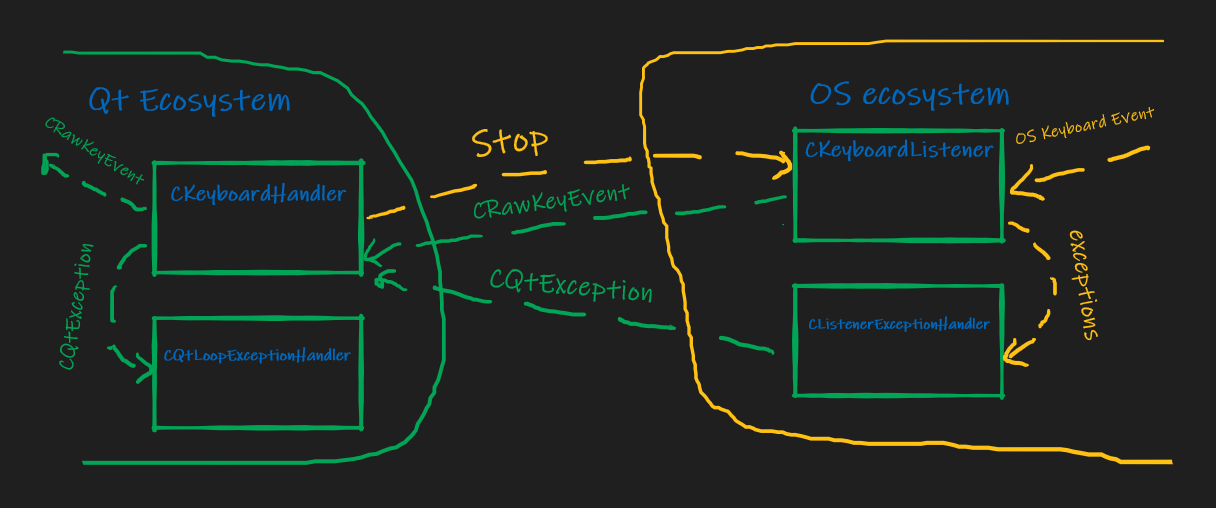
\includegraphics[scale = 0.5]{Figures/KeyboardInterception.png}

Green arrows represent queued Qt signals and yellow arrows represent OS dependent signals.
\end{center}

\subsection{Kernel}

\subsection{Qt Resources}

\subsection{ApplicationImpl}


\section{Code}

\section{Implementation}

\section{Library}
\subsection{Singleton}\label{section::Singleton}
CAnyGlobalAccess template consists of three parts:
\begin{enumerate}
\item \textbf{CAnyGlobalAccessible}. It provides a static storage for a global object. You do not access it directly.
\item \textbf{CAnyGlobalAccess}. This object is used to access the global object. The global object must be initialized before access object is created.
\item \textbf{CAnyGlobalInitializer}. This object is used to initialize the global object. You need to create one instance of this object in order to initialize the global object.
\end{enumerate}
\begin{center}
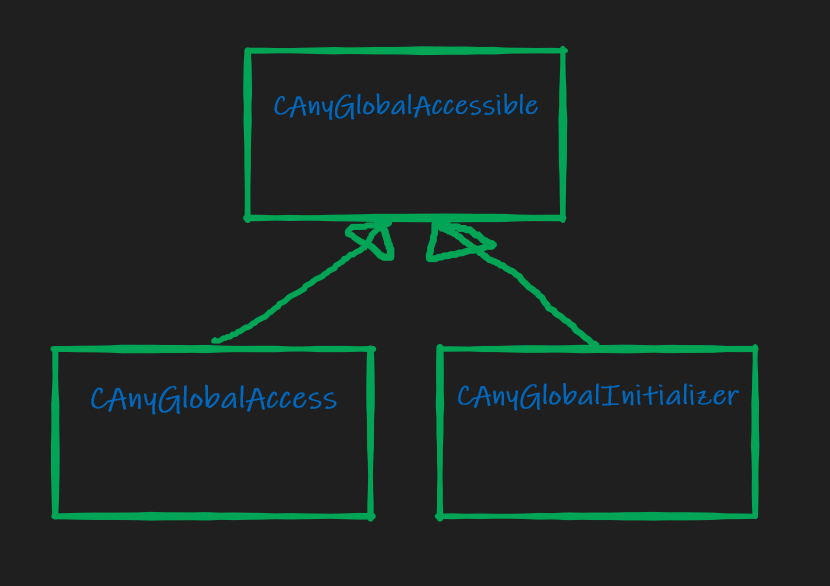
\includegraphics[scale = 0.3]{Figures/CAnyGlobalAccess.png}
\end{center}

\paragraph{Description}
The pattern is used to make a global object with non-trivial constructor without explicitly defining the object globally. \textbf{WARNING} this thing is NOT thread safe! In order to use the pattern we must provide:
\begin{enumerate}
\item \verb"TAccessible" -- the class for the global object

\item \verb"TID" -- identification class. If we want to have several global objects  of a class Type, we must distinguish them by a dummy class \verb"TID". For example, \verb"CAnyGlobalAccessible<Type, A>" and \verb"CAnyGlobalAccessible<Type, B>" store  different instances of objects of type Type in static storage. Since static objects defined by the class they belong to, classes \verb"A" and \verb"B" are required to distinguish the instances.

Example of a dummy class declaration:
\begin{verbatim}
class CGlobalAccessibleID;
\end{verbatim}

\item A class for initialization of the global object. It must be
 inherited from \verb"CAnyGlobalInitializer". The class must inherit all the constructors of the base class.
\begin{verbatim}
class CMyInitializer : CAnyGlobalInitializer<TAccessible, TID> {
   using CBase = CAnyGlobalInitializer<TAccessible, TID>;
 public:
   using CBase::CBase;
 };
\end{verbatim}

\item A class for getting access to the global object must be publicly inherited from \verb"CAnyGlobalAccess". It has only a default constructor. It asserts if  the global object has not yet been initialized.
\begin{verbatim}
class CMyAccessor : public CAnyGlobalAccess<TAccessible, TID> {};
 \end{verbatim}
\end{enumerate}

\paragraph{Example}
Suppose we want a global \verb"int" variable for logging:
\begin{verbatim}
class CLoggerCounterID;
class CLoggerCounterInitializer :
  CAnyGlobalInitializer<int, CLoggerCounterID> {
  using CBase = CAnyGlobalInitializer<int, CLoggerCounterID>;
public:
  using CBase::CBase;
};
class CLoggerCounterAccess : public CAnyGlobalAccess<int, CLoggerCounterID> {};
\end{verbatim}
Then in code we write something like that:
\begin{verbatim}
...
CLoggerCounterInitializer Init(0);
...
CLoggerCounterAccess LogCounter;
++(*LogCounter);
std::cout << *LogCounter << std::endl;
...
\end{verbatim}

\subsection{AnyObject}
\subsubsection{AnyMovable}\label{section::AnyMovable}

\paragraph{Description}
\verb"CAnyMovable" allows you to store any movable only class without any restrictions on the class. It also allows you to provide  an interface to a class and implementations for different classes of the method.

The \verb"operator->()" goes without any checks and may fail if the object is empty, that is, does not store anything. It is your responsibility to call \verb"isDefined()" method before accessing the interface.

The class \verb"CAnyMovable" does not use Small Object Optimization. In particular, move operations are always cheap. \verb"CAnyMovable" has value semantics and extends the ideas of Sean Parent's talk on cppcon about Run-time Polymorphism.

\paragraph{How to use}
In order to use the template you need:
\begin{enumerate}
\item Create an interface class:
\begin{verbatim}
template<class TBase>
class IAny : public TBase {
public:
  virtual void print() const = 0;
};
\end{verbatim}
The class describes the interface of an abstract object you want to support. Do not use names with prefix underscore here, e.g.,
\begin{itemize}
\item[\textbf{BAD}:] \verb"virtual void _print() const = 0;"
\item[\textbf{GOOD}:] \verb"virtual void print() const = 0;"
\end{itemize}
This interface will be accessible when using \verb"operator->()" on \verb"CAnyObject". The example is below.

\item Create an implementation class:
\begin{verbatim}
template<class TBase, class TObject>
class CAnyImpl : public TBase {
  using CBase = TBase;
public:
  using CBase::CBase;
  void print() const override {
    std::cout << "data = " << CBase::Object() << std::endl;
  }
};
\end{verbatim}
Here you implement all the functions from the interface. The parameter \verb"TObject" is used to reimplement the behaviour for different types of objects if needed. In the example above, it may happen that \verb"TObject" does not support stream \verb"operator<<" and you want to define  a specialization of the implementation class. Access to the stored object is provided by the method \verb"CBase::Object()".

\item Create your Any class:
\begin{verbatim}
class CAny : public CAnyMovable<IAny, CAnyImpl> {
  using CBase = CAnyMovable<IAny, CAnyImpl>;
public:
  using CBase::CBase;
  friend bool operator==(const CAny&, const CAny&) {
    ...
  }
};
\end{verbatim}
You can add any additional functionality to your \verb"CAny" class.
\end{enumerate}
Now you can use it like this:
\begin{verbatim}
CAny x = 'c';
x->print();
x = std::move("123");
x->print();
x = 1.45;
x->print();
\end{verbatim}
If you want to store an object of Type \verb"R" and construct it on the fly from the data: \verb"x, y, z". Then use emplace function or emplace constructor like this:
\begin{verbatim}
CAny s;
s.emplace<R>(x, y, z);
CAny y(std::in_place_type_t<R>(), x, y, z);
\end{verbatim}
Then the object of type \verb"R" will be created without creation of intermediate objects.

\paragraph{Implementation}
Internally \verb"CAnyMovable" stores an \verb"std::unique_ptr" to interface \verb"IObjectStored". Let us look at the diagram below:
\begin{center}
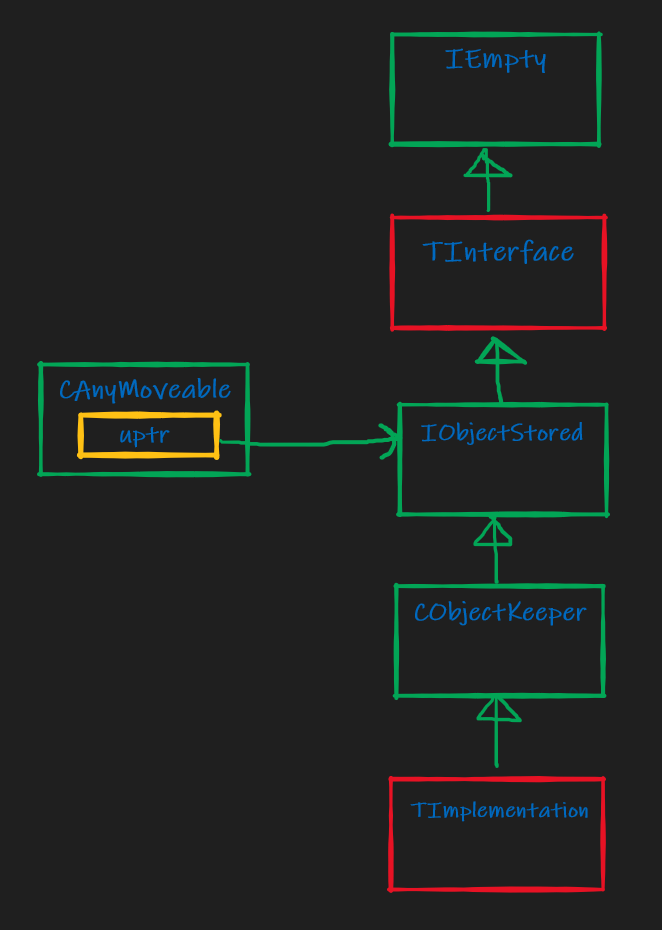
\includegraphics[scale = 0.5]{Figures/CAnyMovable.png}
\end{center}
The red rectangles are templates provided by the user. \verb"IEmpty" is an empty interface with virtual distructor. Its only purpose is to avoid user having to provide a virtual distructor in the \verb"TInterface" template. Then \verb"IObjectStored" adds some virtual methods to provide required functionality. \verb"CObjectKeeper" is a template storing an instance of an object you want to move into \verb"CAnyMovable". \verb"TImplementation" is a user defined template implementing all virtual methods from \verb"TInterface".

\end{document}


